\chapter{Learning Adverse Drug Events}
\section{Introduction}
Adverse drug events (ADEs) are undesired harmful effects resulting
from use of a medication. It is estimated that ADEs occur in 30\% of
hospital stays, causing 2 million injuries, hospitalizations, and
deaths each year in the United States at a cost of \$75 billion
\cite{Classen1997,Classen2011,Lazarou1998}. Pre-approval clinical
trials are the first line of defense for identifying adverse drug
events but they are limited both in their power to detect rare events
and their generalizability to patient populations with poly-pharmacy
and many co-morbidities. These limits have driven efforts in
post-marketing surveillance for ADEs using a variety of observational
data sources as a key component of the learning health care system
\cite{Tatonetti2009,Lependu2013,Harpaz2014,Friedman2009}.

These efforts have at their core the collection of counts of drugs
being taken and adverse events occurring, derived from a variety of
data sources. Most work has used spontaneous reporting system data
such as the US Food and Drug Administration’s FDA Adverse Event
Reporting System (FAERS), but other data sources such as claims data
have also been used. Each of these data sources have well-documented
biases. For instance, FAERS relies on voluntary reporting of suspected
drug adverse event cases and suffers from reporting biases such that
associations with adverse events with many possible causes are
difficult to detect \cite{Harpaz2013}, while claims data suffers from
biases arising from its primary use for billing instead of conveying
clinical information \cite{Ryan2013}.

In contrast, the electronic medical record (EMR) and free text of
clinical notes provides arguably the most complete and unbiased
picture of clinical events available \cite{Poissant2010}. There has
been much progress in using methods from Natural Language Processing
(NLP) to extract structured information from the unstructured free
text of clinical notes \cite{Wang2009,Lependu2013}. These studies
typically use Natural Language Processing (NLP) to generate counts of
drug and disorder mentions in the clinical text, often subject to
constraints that reflect, for instance, the intuition that the cause
of an adverse event, e.g., taking a drug, must precede the adverse
event itself. Given such counts, there are two main approaches to
identifying possible drug adverse event associations. One approach,
disproportionality analysis (DPA), tackles the problem using the
well-known framework of statistical hypothesis testing
\cite{Harpaz2013}. These methods use counts of drugs, adverse events,
and their co-occurrence to calculate a p-value for the association of
the drug and adverse event relative to a null hypothesis of no
association, with varying degrees of adjustment for
confounding. However, recent work has shown that using p-values to
prioritize possible drug-adverse event associations is problematic
\cite{Schuemie2014}. Furthermore, it has been noted that integration
of other data sources is likely essential in effective post-marketing
surveillance using observational data \cite{Ryan2013}. However, it is
not clear how to effectively incorporate some forms of relevant
information, such as prior knowledge of known ADEs. Such prior
knowledge may be especially helpful for detection of ADEs in which the
drug or adverse event is rare.

An alternative to statistical hypothesis testing is using
discriminative classifiers such as a logistic regression model. These
methods differ from DPA in that they attempt to learn a function that
guesses the validity of drug adverse event associations given inputs,
or features, such as counts of the drug and the adverse event in the
data. Importantly, the input can include features that reflect prior
knowledge such as similarity to known adverse drug events. Such
discriminative classifiers can be applied to spontaneous reports or to
EMR derived counts. Harpaz et al \cite{Harpaz2013} conducted a
systematic review of drug adverse event algorithms using FAERS data
that found logistic regression methods outperforming state of
the art DPA methods across a variety of adverse events. Recent work by
Noren et al has shown that building such a discriminative classifier
that uses additional information such as the geographic origin of an
adverse event report and the timing of the submission achieves much
better performance than existing methods
\cite{Caster2014,Caster2013,Harpaz2013b}. Cami et al \cite{Cami2011}
went even further and developed a logistic regression model using only
features encoding prior knowledge about known ADEs that achieved high
performance.  Liu et al \cite{Li2011} used a discriminative classifier
to distinguish adverse drug events (pairs of drugs and adverse events
in which the drug causes the adverse event) from drug usages (pairs of
drugs and disorders in which the drug is used to treat the
disorder). Their classifier used features derived from the free text
of millions of clinical notes from the Stanford Translational Research
Integrated Database Environment (STRIDE) \cite{Lowe2009} that encoded
the frequency of drug and disorder mentions and co-mentions in the
text, subject to constraints on the order of the mentions in
time. However, this preliminary work simply evaluated the performance
of the classifier using cross validation and did not attempt to
discover novel drug adverse event associations. It also restricted
itself to drug-disorder pairs in which both the drug and disorder were
frequently mentioned together, limiting its utility for detecting rare
AEs. In related work, Jung et al \cite{Jung2014} used EMR derived
features to detect drug usage pairs, but also added additional
features encoding prior knowledge about known drug usages. These
additional features were found to significantly improve the
performance of the classifier in a validation set, and the classifier
was applied to all possible drug and indication pairs to identify
putative off-label drug usages.

We have built on this work, developing a method suited for systematic,
automated detection of potential adverse drug events from the EMR. Our
method uses the text from clinical notes, along with prior knowledge
of drug usages and known adverse drug events, as inputs. We use a
computationally efficient text processing system to extract mentions
of drugs and disorders from the text. These mentions are further
processed into statistics that are used by a discriminative classifier
that outputs the probability that a given drug-disorder pair
represents a valid adverse drug event association. The classifier
achieved an area under the ROC curve (AUC) of 0.94 on hold out test
data. Applying it to all possible drug-adverse event pairs and
filtering the predicted ADEs support in independent and complementary
data sources – FAERS and MEDLINE – resulted in 240 high-confidence
ADEs. Figure 3.1 summarizes our approach.

\begin{figure}
  \begin{center}
    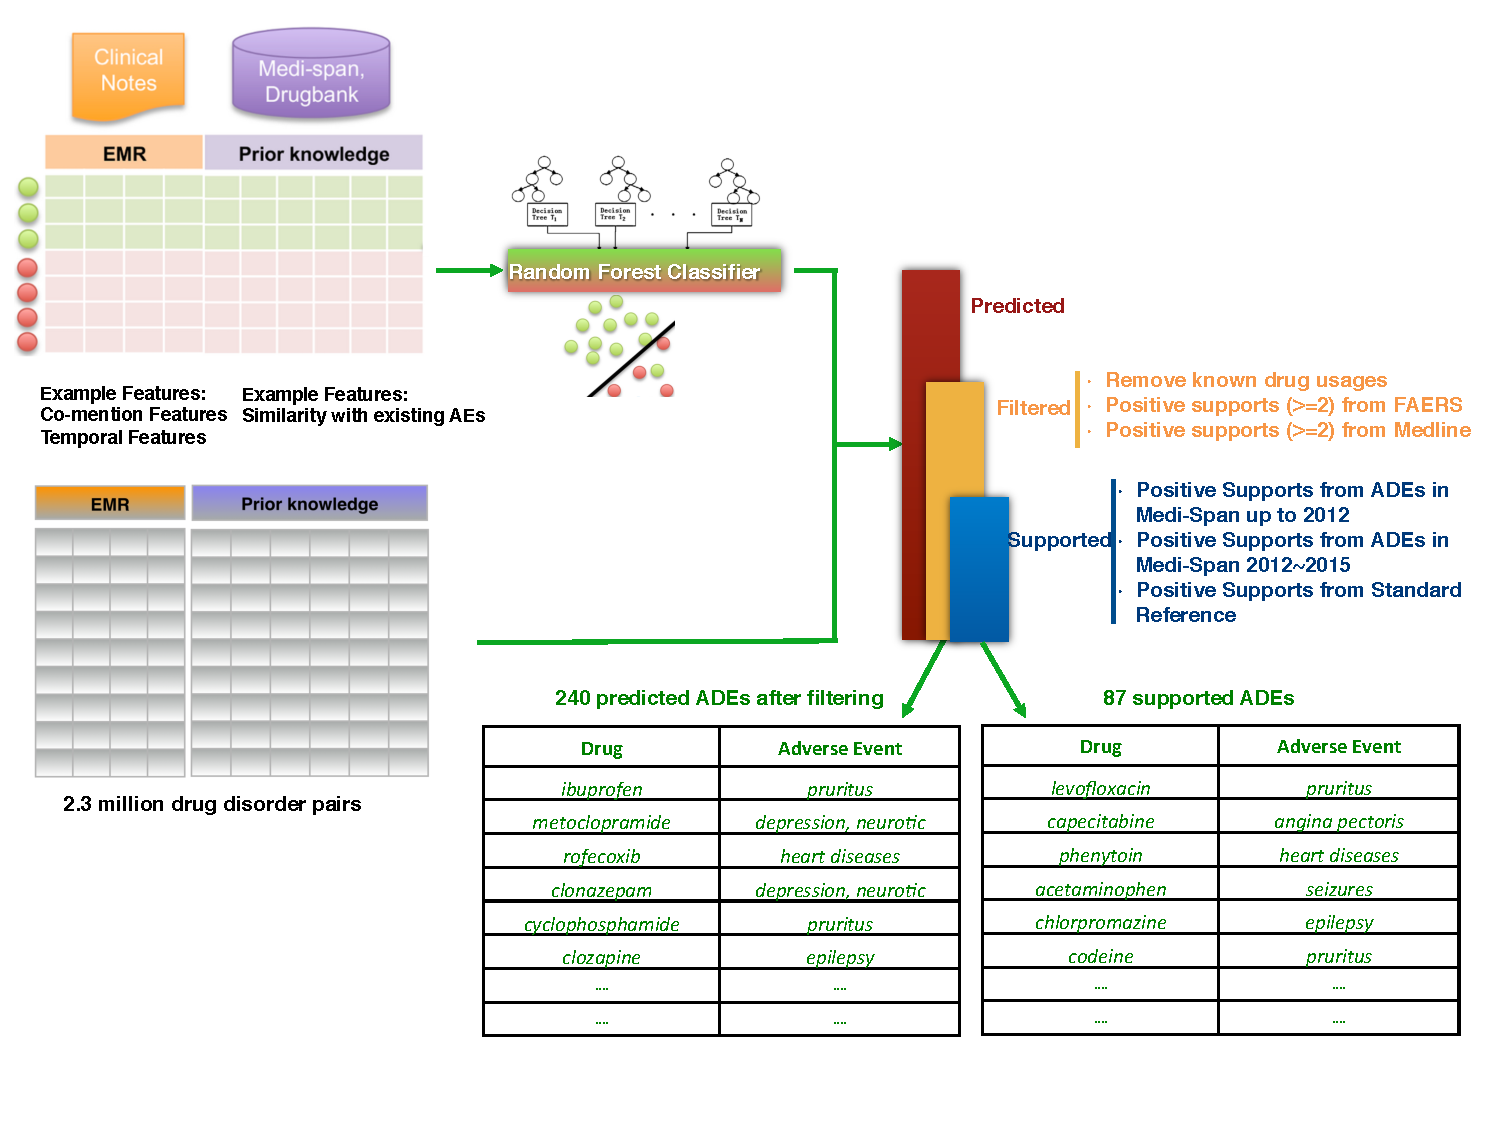
\includegraphics[width=0.9\linewidth]{ch3-figures/Figure1.pdf}
  \end{center}
  \caption[Feature engineeering for ADE discovery]{For each of the
    2,362,950 possible drug-disorder pairs, we calculated 9 features
    from the free text of clinical notes in STRIDE, 8 features from
    known AEs in Medi-Span, and 12 features from known usages in
    Medi-Span and Drugbank. Based on these features, a Random Forest
    classifier was trained on the gold standard dataset to recognize
    the drug-AE relationships. Then, we applied the trained
    classifiers to the possible drug-disorder pairs and
    filtered for support in FAERS and MEDLINE, yielding a set of 240
    predicted ADEs. Drug-AE pairs used in training are also removed.  }
  \label{fig:short}
\end{figure}


\section{Materials and Methods}
\subsection{Constructing training and test sets}
Discriminative classifiers learn a function that maps input features
to an output such as the probability that the inputs represent a true
drug adverse event pair. In order to learn and evaluate the
performance of this function, these methods require a set of examples
of drug adverse event pairs whose status as true or false associations
is known. We constructed such a set of positive and negative examples
of drug-AE pairs using known ADEs from Medi-Span® Adverse Drug Effects
Database (from Wolters Kluwer Health, Indianapolis, IN). Medi-Span up
to 2012 contains 711,468 drug-disorder pairs comprising 13,000 unique
drugs and 3,403 unique disorders. Of these, 3,550 pairs were assumed
to be true adverse drug event pairs because they occur in black box
warnings with additional constraints (e.g. above moderate severity
level). We used RxNorm to normalize drugs to their active ingredients
and discarded pairs in which either the drug or adverse event did not
occur in the EMR data. This resulted in 1,898 positive examples for
training and testing. To construct negative examples, we randomly
sampled drugs and adverse events from among the drugs and adverse
events in the positive set and ensured that the co-mention counts
distribution of the negative samples are roughly the same as those of
the positive samples. 4,336 such negative samples remained after
removing inadvertently generated positive examples. These drug adverse
event pairs were then randomly split into 4,358 training examples used
to learn classifiers and 1,877 test examples used to evaluate the
performance of the classifiers.

\subsection{Processing of clinical text-notes from STRIDE}
An NCBO Annotator based text-processing pipeline
\cite{Lependu2012,Jung2014b} was used to annotate 9.5 million clinical
notes from STRIDE with mentions of drugs and disorders. Negated
mentions (e.g., “MI was ruled out”) or those referring to other people
(e.g., “father had a stroke”) were removed using NegEx
\cite{Chapman2001} and ConText \cite{Chapman2007}, respectively.  The
notes spanned 18 years and 1.6 million patients. Drugs and disorders
were mapped to UMLS unique concept identifiers (CUIs). In this study
we used the 2011AB version of the UMLS. Drugs were normalized to
active ingredients using RxNorm \cite{Nelson2011} as provided by
UMLS2011AB – for example, Panocaps was normalized to lipase, protease,
and amylase.

\subsection{Feature construction}
For each drug-disorder pair, we constructed nine features from the
clinical note derived mentions – the drug and disorder frequency,
co-mention frequency, drug first fraction (the fraction of patients in
which the first mention of the drug precedes the first mention of the
disorder) and association scores derived from these counts (e.g., chi
squared statistic, odds ratio, and the conditional probability of drug
mention given disorder mention).

In addition, we constructed eight features encoding known drug-AEs and
twelve features encoding known usages. Those features were motivated
by the intuition that a drug may be more likely to cause an adverse
event if similar drugs are known to cause that adverse event. Known
AEs were defined as appearing in Medi-Span. For each drug-disorder
pair, we computed the similarity of the drug to drugs known to cause
the disorder, and the similarity of the disorder to other disorders
caused by the drug. The calculation of drug-drug and disorder-disorder
similarity is described in Figure 3.2. For usage-similarity, we
adopted features described in Jung et al \cite{Jung2014}. In all, we
used 29 features for each drug-disorder pair.

\begin{figure}
  \begin{center}
    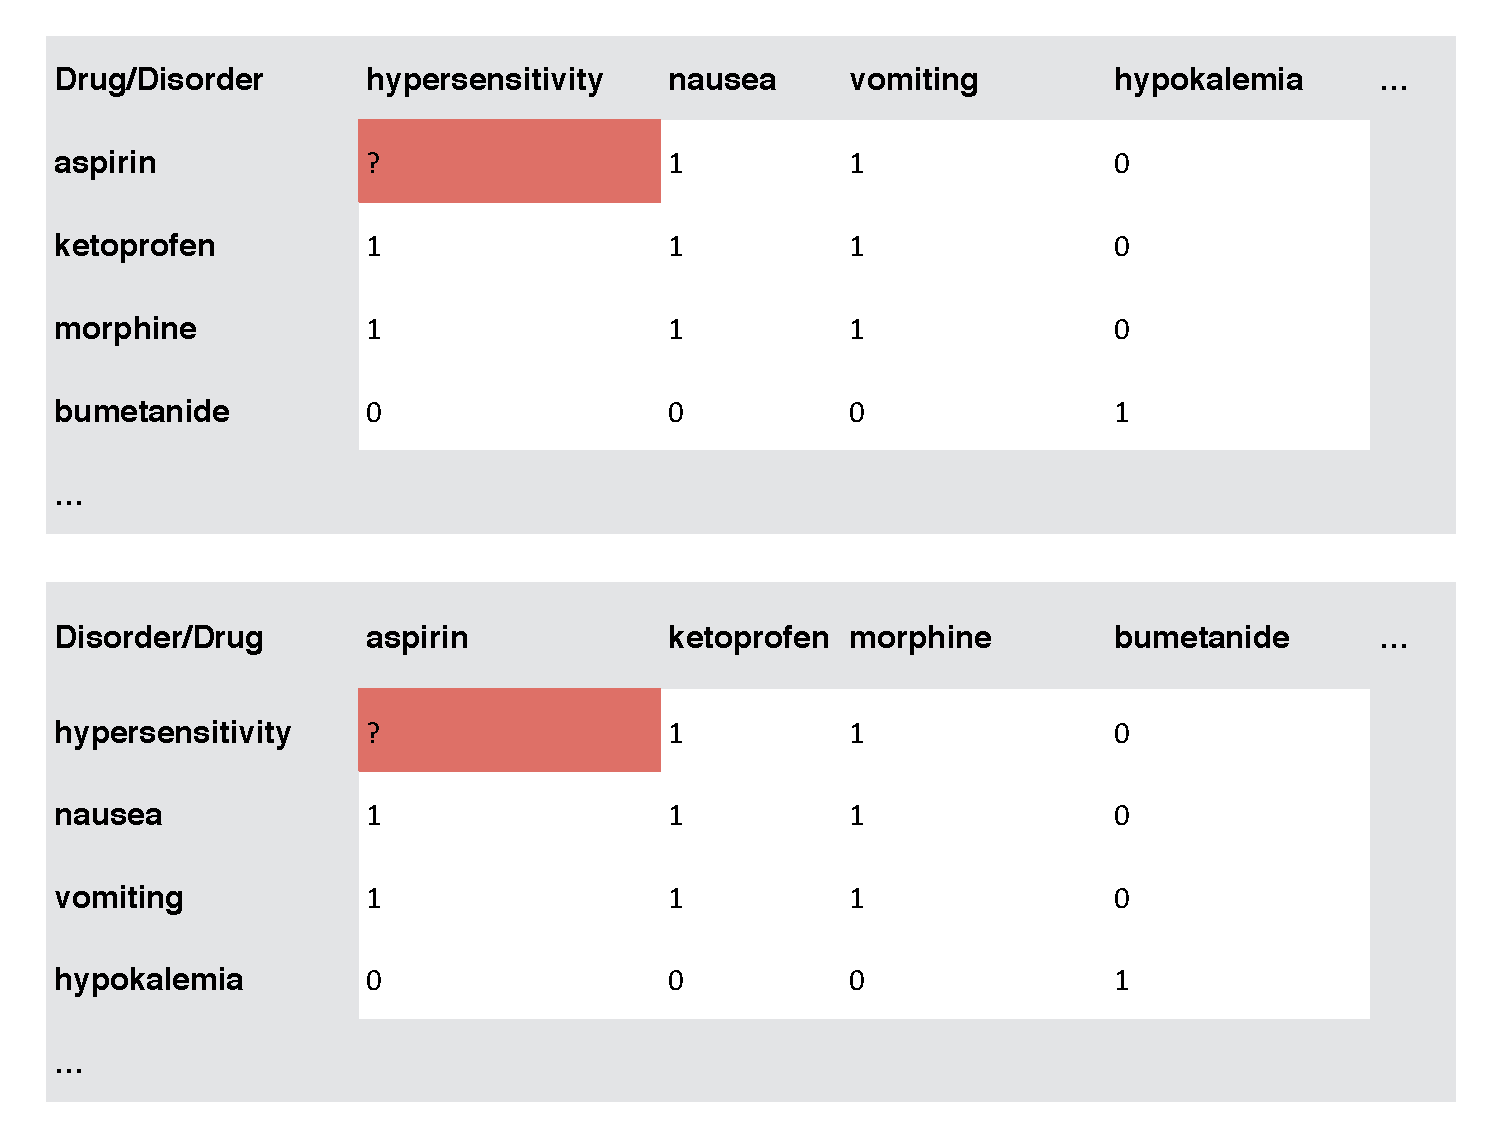
\includegraphics[width=0.9\linewidth]{ch3-figures/Figure2.pdf}
  \end{center}
  \caption[Calculating drug-drug and disorder-disorder similarity]{
    We represent prior knowledge about ADEs as matrices in which each row is a
    drug and each column is an AE.  The (i,j)-th entry is an indicator
    for whether or not the drug i is known to be associated with AE
    j.  We are interested in computing a feature that captures the
    intuition that drugs with similar adverse event profiles are more
    likely to also be associated with a new, unknown adverse event.
    Say we are interested in the associationn of drug i with AE j.  We
    first find other drugs which are \emph{known} to be associated
    with AE j.  We then compute the similarity of drug i with all of
    these drugs using cosine and Jacquard similarity.  These
    similarities are then pooled over the set of other drugs by using
    the max and the mean.  To calculate drug-drug similarity with
    respect to other characteristics such as targeted molecular
    pathways from Drugbank, we simply use a matrix in which the
    columns represent pathways.  To calculate disorder-disorder
    similarity, we perform an analogous calculation with the roles of
    drugs and AEs reversed.}
  \label{fig:short}
\end{figure}


\subsection{Classifier development}
We fit L1 regularized logistic regression (lasso) \cite{Lasso}, SVM
with radial basis function kernel \cite{SVM} , and random forest
classifiers \cite{Liaw2002} to the training data. Model
hyperparameters were fit by cross validation in the training data.
The classifiers were then evaluated on the hold out test set. The
classifier development process is summarized in Figure 3.3. In order
to investigate the contribution of different features, we performed an
ablation analysis in which we evaluated classifiers using subsets of
the features.

\begin{figure}
  \begin{center}
    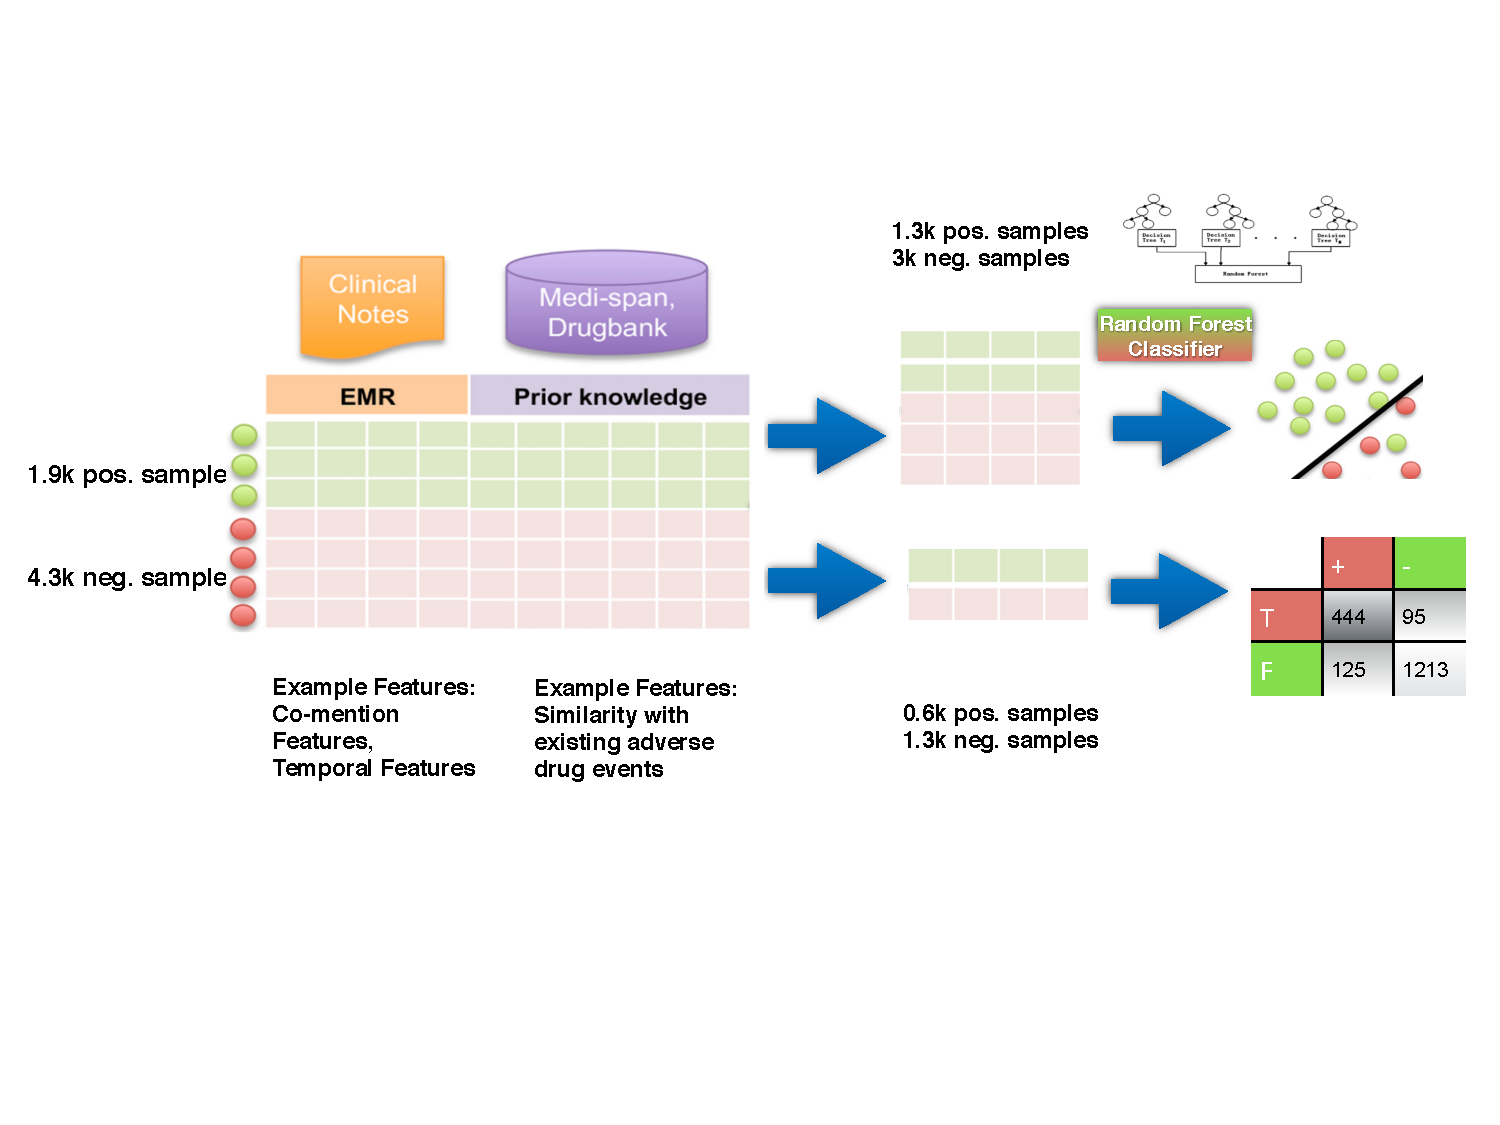
\includegraphics[width=0.9\linewidth]{ch3-figures/Figure3.pdf}
  \end{center}
  \caption[Training a classifier to recognize ADEs]{Positive examples
    collected from known drug AEs in Medi-Span and negative examples
    created through randomly sampling a drug and disorder with roughly
    the same co-mention distribution as the positive examples. For
    each drug-disorder pair in the gold standard, we used 9 features
    to characterize the pattern of drug and disorder mentions in 9.5
    million clinical notes from STRIDE, 8 features to characterize the
    domain knowledge of drug, disorder, and known AEs from Medi-Span,
    and 12 features to characterize the domain knowledge of drug,
    disorder, and known usages from Medi-Span and Drugbank. The gold
    standard dataset was randomly split into 70\% for training and
    30\% for testing the classifier.}
  \label{fig:short}
\end{figure}


\subsection{Identifying putative drug-AE associations}
Performance on the test set indicated that the random forest
classifier was superior to the other classifiers in all metrics. We
therefore focused on this model and applied a classifier trained on
the full gold standard dataset to the 2,362,950 possible drug-AE pairs
comprised of 1,602 unique drugs and 1,472 unique disorders appearing
in our data. We focused on the most confident predicted associations
by using a threshold of 0.7 for the posterior probability output by
the classifier, yielding 41,248 predicted ADE associations.  Known
ADEs and drug usages were then filtered out.  In this study, the set
of 3,550 known ADEs were gathered from the Medi-Span® Adverse Drug
Effects Database, where the documentation level is marked as “black
box warning”; known usages were gathered from the Medi-Span Drug
Indications Database (Wolters Kluwer Health, Indianapolis, IN) and the
National Drug File – Reference Terminology (NDF-RT) \cite{Brown2004}.

\subsection{Filtering in FAERS and MEDLINE}
We filtered the drug-AE associations using FAERS \textbf{REF} and
MEDLINE, two independent and complementary data sources that reflect
clinical practice and published biomedical knowledge
respectively. FAERS case reports contain explicit links between drugs
and adverse events. We used all case reports from Q1 2005 through Q4
2013 to assess support for putative ADEs in terms of the number of
case reports in which the drug was reported as the primary or
secondary suspect drug for the adverse event. FAERS drugs and adverse
events were mapped to UMLS CUIs, yielding a set of 4,508,892
drug-event reports covering 372,379 unique pairs. We also obtained
reports of adverse drug events described in the biomedical literature
from MEDLINE. Using an approach described by Winnenburg et al
\cite{Winnenburg2015}, we obtained 118,552 unique ADEs from about
200,000 articles in MEDLINE that had been manually annotated with
combinations of Medical Subject Heading (MeSH) descriptors and
qualifiers for both a drug involved in an adverse event (e.g.,
Ofloxacin/adverse effects) and its manifestation (e.g.,
Tendinopathy/chemically induced). We mapped the MeSH terms of drug -
disease pairs (e.g., Ofloxacin – Tendinopathy) to their corresponding
UMLS CUIs to make the findings compatible with our predictions.

\subsection{Validation in Medi-Span and Time-Indexed Reference}
We validated the drug-AE associations using future years of data from
Medi-Span. The training examples used in our model were constructed
from ADEs marked as “black box warning” in Medi-Span up to 2012—thus
we only used well-established adverse events in training the
classifier. Medi-Span also contains ADEs marked as “reported in
multiple reports and uncontrolled studies” or “reported in few case
reports and suggested links”; we refer to these ADEs with moderate
support.  We validated the drug-AE associations left after filtering
based on FAERS and MEDLINE using ADEs with moderate support in both
Medi-Span up to 2012 as well as with the additional Medi-Span data
from 2012 to 2015.  Medi-Span up to 2012 contains 95,115 ADEs with
moderate support, and Medi-Span from 2012 to 2015 contains an
additional 755 ADEs that were not reported in Medi-Span as of 2012. In
addition, we used a time-indexed reference standard by Harpaz, R. et
al. \cite{Harpaz2013b} to further assess the classifier’s ability to
detect recent drug-AE associations. The reference standard was
systematically curated from drug labeling revisions (e.g. new warnings
issued and communicated by the US Food and Drug Administration in
2013), and included 62 positive test cases and 75 negative controls.

\subsection{Feature contribution}
We performed feature ablation experiments to investigate whether or
not our encoding of domain knowledge contributed to model
performance.  We grouped the twenty-nine features into
three categories: features from Clinical Notes (CN), features from
known AEs (KA), and features from known usages (KU).  Classifiers were
trained on each of these subsets of features, along with the
combinations CN+KA and CN+KU.  The performance of these models were
then evaluated on the test set. 

\section{Results}
\subsection{Performance of the classifier}
The random forest classifier to detect drug-AE associations achieved
an AUC of 0.94 in a hold out test set. We then fit a new random forest
classifier using the entire gold standard and applied it to the
2,362,950 drug-AE pairs arising from 1,602 unique drugs and 1,472
unique disorders appearing in our data. After applying a cutoff on the
classifier’s confidence (posterior probability of 0.7), we arrived at
a set of 41,248 putative drug-AE associations. We refined these 41,248
drug-AE associations by filtering for support in FAERS and
MEDLINE. 240 associations were supported by at least 2 reports in both
FAERS and MEDLINE. Table 3.1 lists the ten associations with the
highest level of support in FAERS.

\begin{table}
\begin{center}
\begin{tabular}{|c|c|c|c|c|c||}
  \hline Drug Name & Drug CUI & Event Name & Event CUI & FAERS &
  MEDLINE \\ & & & & Support & Support \\ \hline\hline etanercept &
  C0717758 & pruritus & C0033774 & 11485 & 2 \\ metoclopramide &
  C0025853 & depression, neurotic & C0282126 & 1473 & 9 \\ rofecoxib &
  C0762662 & heart diseases & C0018799 & 861 & 3 \\ clonazepam &
  C0009011 & depression, neurotic & C0282126 & 691 & 2 \\ diazepam &
  C0012010 & depression, neurotic & C0282126 & 608 & 5 \\ levofloxacin
  & C0282386 & pruritus & C0033774 & 540 & 3 \\ cyclosporine &
  C0010592 & pruritus & C0033774 & 517 & 5 \\ clozapine & C0009079 &
  epilepsy & C0014544 & 410 & 13 \\ lorazepam & C0024002 & depression,
  neurotic & C0282126 & 403 & 3 \\ ibuprofen & C0020740 & pruritus &
  C0033774 & 374 & 4 \\ \hline
\end{tabular}
\end{center}
\caption[Ten validated ADEs and their support in FAERS and
  MEDLINE]{List of ten validated Drug-AEs and their support in FAERS
  as well as MEDLINE}
\end{table}

\subsection{Contribution of feature sets}
We evaluated the performance of models trained on subsets of the
features to investigate their contribution to model performance.  The
results are summarized in Table 3.2.  Classifiers using features from
clinical notes, known AEs, and known usages had AUCs of 0.92, 0.72 and
0.82 respectively. Classifiers that used both clinical note features
and known ADE or usage information achieved an AUC of 0.93. Above the
features derived from clinical notes, features from prior knowledge
contributed little in our classifier. Thus, it may be helpful to
incorporate the features used in Cami et al’s in the model. Adding
features from known AEs or known usages to features from clinical
notes significantly improved the classifier performance in terms of
sensitivity, while all features together resulted in a sensitivity of
0.839 and an AUC of 0.944.

\begin{table}
\begin{center}
\begin{tabular}{|c|c|c|c|c||}
  \hline Feature set & AUC & PPV & Specificity & Recall
  \\ \hline\hline Clinical Notes (CN) & 0.920 & 0.763 & 0.803 & 0.702
  \\ Known Adverse-Event (KA) & 0.723 & 0.526 & 0.624 & 0.550 \\ Know
  Usage (KU) & 0.815 & 0.561 & 0.661 & 0.584 \\ CN+KA & 0.932 & 0.775
  & 0.714 & 0.801 \\ CN+KU & 0.937 & 0.781 & 0.719 & 0.820 \\ ALL &
  0.944 & 0.796 & 0.913 & 0.839 \\ \hline
\end{tabular}
\end{center}
\caption[Performance of ADE classifier]{Performance of Random Forest
  classifier on held-out test set with different feature sets}
\end{table}


\subsection{Assessing the quality of the predictions}
Out of the 240 well-supported drug-AE associations, 76 occurred in the
set of the ADEs with moderate support in Medi-Span up to 2012. We also
found that 10 out of the 240 drug-AE associations occurred in the
recent established ADEs included in the additional Medi-Span data from
2012 to 2015. Finally, two of the drug-AE associations were also
supported by the reference standard provided by Harpaz, R. et al.
Figure 3.4 shows the support from those data sources for the predicted
drug-AE associations. Overall, from the 240 drug-AE associations, 87
of them (36\%) are supported in at least one of the resources that
have information not available to the classifier.

\begin{figure}
  \begin{center}
    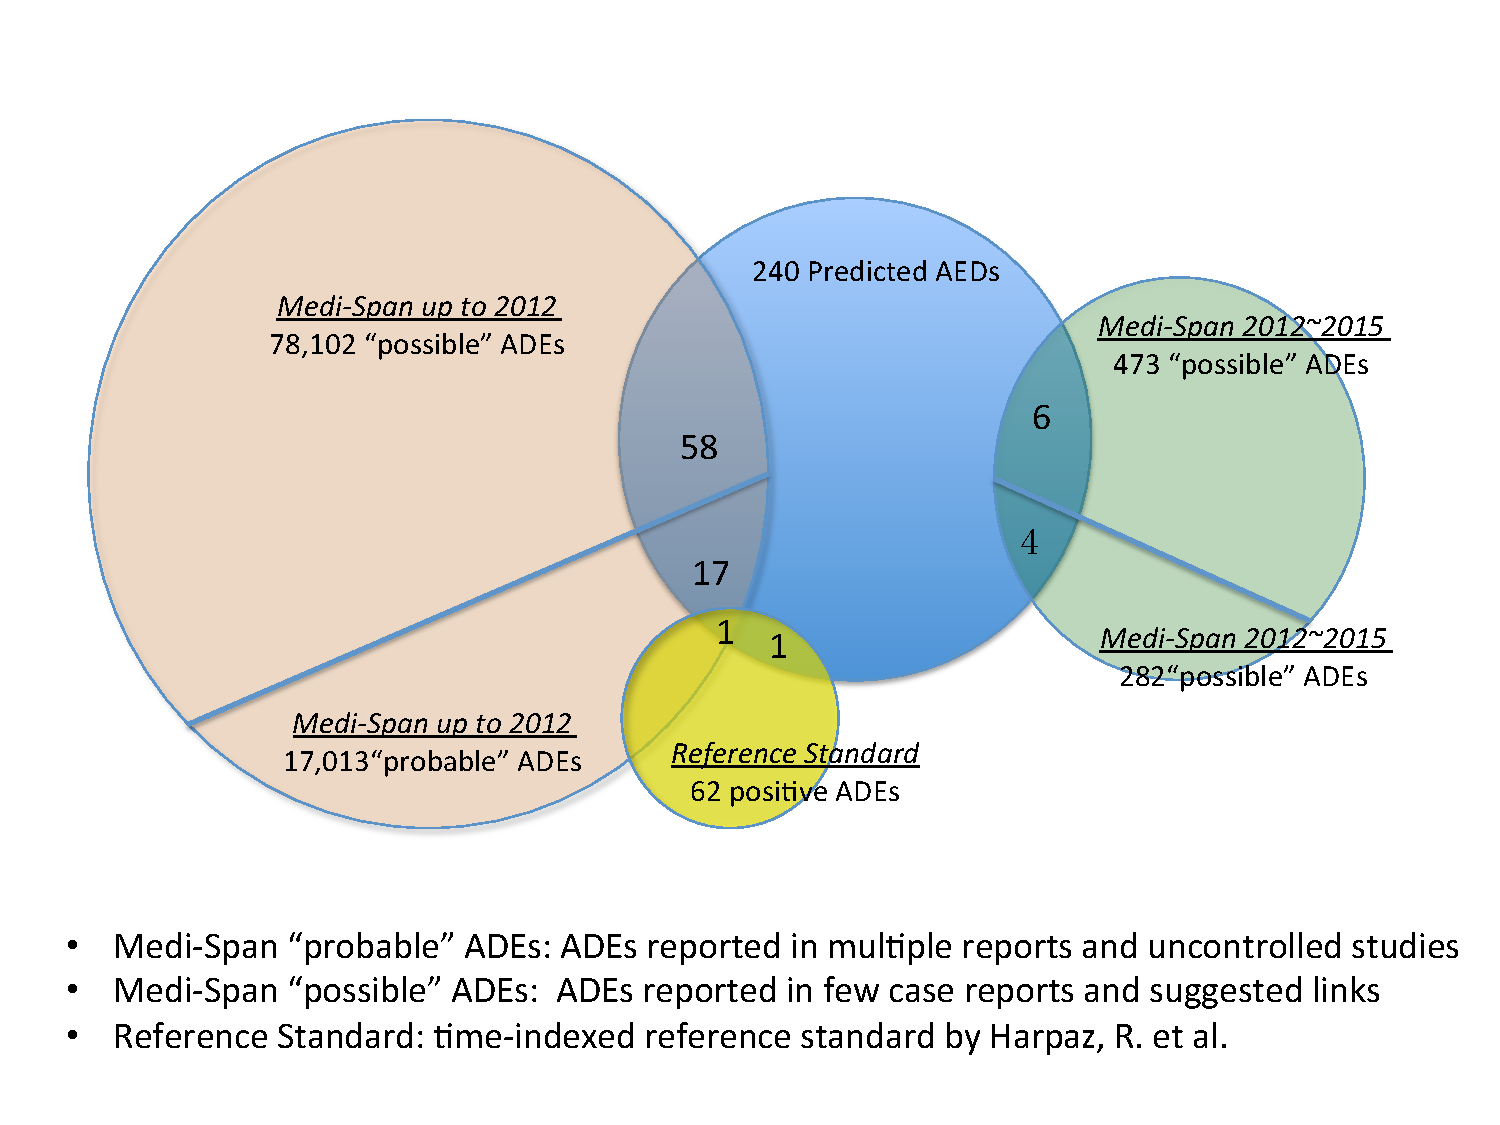
\includegraphics[width=0.9\linewidth]{ch3-figures/Figure4.pdf}
  \end{center}
  \caption[Validation of predicted ADEs]{We validated the predicted
    drug-AE associations from three independent and complementary data
    sources. From the 240 drug-AE associations, 76 occurred in the set
    of the ADEs with moderate support in Medi-Span up to 2012; 10
    occurred in the recent established ADEs included in the additional
    Medi-Span data from 2012 to 2015; two occurred in the reference
    standard provided by Harpaz, R. et al. Overall, 87 of them (36\%)
    were supported in at least one of the resources which have
    information that was not available to the classifier.  }
  \label{fig:short}
\end{figure}


\section{Discussion}
We have developed a method for systematic, automated detection of
adverse drug events. The method achieves high specificity and
sensitivity in a hold out test set using features derived from both
clinical notes and prior knowledge about drug usages and adverse drug
events. Our classifier does not make any assumptions on relationship
between the inputs, allowing us to easily incorporate disparate types
of knowledge into the predictions. In particular, features derived
from clinical notes are empirical, and reflect clinical practice as
is, while features encoding prior knowledge potentially allow us to
make better predictions in cases where the empirical data is lacking.
The direct use of EMRs also opens the door to prioritizing potential
novel ADEs using the observed frequency of co-occurrence of the drug
and adverse event in the EMR, which may better reflect their true
prevalence than data sources such as FAERS. We note that systematic
detection of adverse drug events requires methods that are easily
applicable to many health care institutions. Our method has several
characteristics that make it especially suitable for such use. First,
its input is primarily derived from clinical free text through a
computationally efficient text processing system that can handle
millions of notes in hours. Second, unlike other approaches to
enabling cross institution analysis of EMR data, our method assumes
only access to the text of clinical notes without assuming a common
data model. Third, it is easy to adapt the classifier to different
institutions because no components other than the classifier need site
specific tuning. The latter is not an obstacle to adoption because the
training and validation of the classifier can be entirely
automated. These characteristics of our approach minimize the
computational and organizational demands of implementing the method in
a variety of settings.  Our work has important limitations. First, we
emphasize that the classifier generates hypotheses (i.e. “signals” of
a putative association) instead of verified ADEs. Furthermore, our
working definition of novelty in this study is novelty with respect to
a set of well-established ADEs. We view this positively, as further
validation of our method, because our primary aim is to demonstrate
the feasibility of an approach to post-marketing surveillance which is
suitable for large scale deployment across many health care
institutions. We note that in practice, the set of ‘known ADEs’ used
in training could be tuned to change the sensitivity of the
classifier. We also note that despite the classifier’s high
specificity in test data, applying it to millions of hypothetical
drug-AE pairs may result in a large absolute number of false
positives. Second, as in previous studies that have used free text to
discover relationships between drugs and disorders, the mismatch
between terms as they are formally defined in formal ontologies versus
how they are used in practice may lead to seemingly novel results that
in fact already known \cite{Jung2014}. Third, we note that while the
use of clinical notes may provide an estimate of prevalence that can
be used to prioritize findings for further study, it would be better
still to combine prevalence with severity, which may require deeper
natural language processing to ascertain severity. Finally, we note
that any biases that are present in the training set of known ADEs
will likely carry over to predictions made on a wider range of drug
adverse event pairs, potentially leading to missed
associations. Furthermore, with respect to the use of this method for
systematic, nation-wide post-marketing surveillance, we note that the
problem of optimally integrating safety signals from multiple sites is
an unsolved research problem despite recent progress
\cite{Harpaz2013c}. Meta-analysis approaches of weighted voting
schemes are necessary to combine the signals generated by such a
classifier from multiple sites.  Despite these limitations, this
method is an important first step towards automated, systematic and
comprehensive post-marketing surveillance for ADEs using electronic
medical records as the primary source; such ability is an important
use case envisioned for the learning health care system [10]. We
envision a future in which it is possible to generate hypotheses of
adverse drug events automatically, in real time, and queue them up for
potential review and submission to the Federal Adverse Event Reporting
System.

\section{Conclusion}
We have developed and validated a data-mining method for identifying
putative, new adverse drug events using clinical data and prior
knowledge of known ADEs. Our classifier achieves high discrimination
capability with an AUC of 0.94 on a held out test set. By applying the
classifier to 2,362,950 drug-disorder pairs consisting of 1,602 unique
drugs and 1,472 unique disorders we identified 240 high-confidence
drug-AE associations. These high-confidence associations are well
supported by multiple independent and complementary resources. Our
method enables systematic post-marketing surveillance for new ADEs
using EMRs.

